\vspace*{\subsecspace}
\section{SciSpot Experimental Evaluation}
%\section{Model Testing and Validation}
%\section{Testing and Evaluation of Model-Informed Policies}
%\section{Model and Policy Evaluation}
\label{sec:eval}

%%\vspace*{\subsecspace}
%\section{SciSpot Design and Implementation}
\subsection{Details of the Experimental Framework used for Evaluation}
%\section{Model-Informed Policy Implementation}
\label{sec:impl}


\sysname is a general-purpose software framework for running scientific computing applications on low-cost transient cloud servers.
It incorporates policies and mechanisms for generating, deploying, orchestrating, and monitoring bags of jobs on cloud servers.
Specifically, it runs a bag of jobs defined by these parameters:
\begin{lstlisting}[basicstyle=\sffamily, frame=single, columns=fullflexible, escapeinside={(*}{*)}]
  Bag of job = {(*$\mathcal{A}$*): Application to execute,
  (*$n$*): Number of jobs,
  (*$m$*): Minimum number of jobs to finish,
  (*$\pi$*): Generator function for job parameters,
  (*$\mathcal{R}$*): Computing resources per job}
\end{lstlisting}


%Additionally, ease-of-use is one of \sysname's primary design goals, and we specifically incorporate

%it is suitable for running a large variety of applications.
\sysname seeks to minimize the cost and running time of bags of jobs of scientific computing applications.
\sysname's cost and time minimizing policies for running bags of jobs are based on empirical and analytical models of the cost and preemption dynamics of  transient cloud servers, which we present in the next section. 

\sysname is designed as a framework that increases the usability and viability of transient cloud servers for scientific computing applications, and provides a simple user interface to allow users to deploy their applications with minimum workflow changes. 
Most scientific computing applications are deployed on HPC clusters that have a batch scheduler such as Slurm~\cite{slurm} or Torque~\cite{torque}, and \sysname integrates with these schedulers (e.g., Slurm) to provide the same interface to applications. 
As shown in Figure~\ref{fig:arch},
\sysname creates and manages clusters of transient cloud servers, manages all aspects of the VM lifecycle and costs, and implements the various policies described in the rest of this section. 

\begin{figure}[t]
  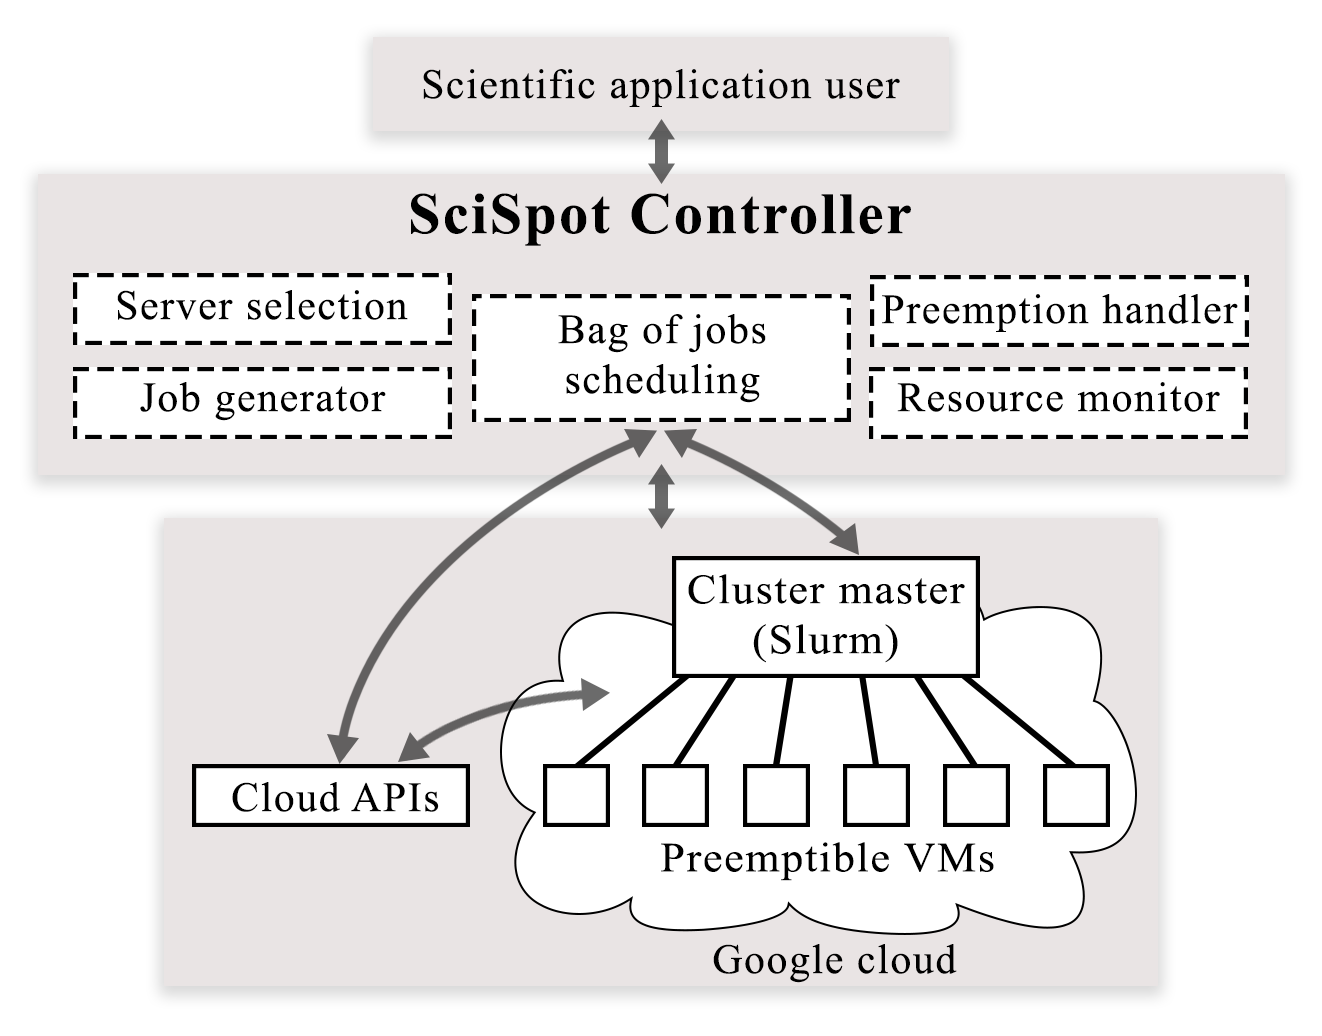
\includegraphics[width=0.3\textwidth]{../figures/Architecture.png}
\vspace*{\myfigspace}
  \caption{SciSpot architecture and system components.}
  \label{fig:arch}
  \vspace*{\myfigspace}
\end{figure}


\noindent \textbf{High-level workflow:} When a user wishes to run a bag of jobs, \sysname handles the provisioning of a cluster of transient cloud servers.
In addition, \sysname deals with the scheduling and monitoring of the bag of jobs, and with VM preemptions. 
Execution of a bag of jobs proceeds in two phases.
In the first phase, \sysname selects the ``right'' cluster configuration for a given application through a cost-minimizing exploration-based search policy, described in Section~\ref{subsec:server-selection}. 
In the second phase, \sysname proceeds to run the remaining jobs in the bag on the optimal cluster configuration. 

\prat{End design}


\sysname is implemented as a light-weight, extensible framework that makes it convenient and cheap to run scientific computing applications in the cloud.
We have implemented the \sysname prototype in Python in about 2,000 lines of code, and currently support running VMs on the Google Cloud Platform~\cite{gcp}. 
%
\sysname is implemented as a centralized controller, which implements the VM selection and job scheduling policies described in Section~\ref{sec:design}. 
The controller can run on any machine (including the user's local machine, or inside a cloud VM), and exposes an HTTP API to end-users. 
Users submit bags of jobs to the controller via the HTTP API, which then launches and maintains a cluster of cloud VMs, and maintains the job queue and metadata in a local database. 
To improve usability, we automatically generate parameter combinations for a given bag size, based on a user-provided json file with ranges and constraints for each parameter. 

\sysname integrates, and interfaces with two primary services.
First, it uses the Google cloud API~\cite{gcloud-api} for launching, terminating, and monitoring VMs.
Once a cluster is launched, it then configures a cluster manager such as Slurm~\cite{slurm} or Torque~\cite{torque}, to which it submits jobs. 
\sysname uses the Slurm cluster manager, with each VM acting as a Slurm ``cloud'' node, which allows Slurm to gracefully handle VM preemptions.
The Slurm master node runs on a small, 2 CPU non-preemptible VM, which is shared by all applications and users. 
\sysname monitors job completions and failures (due to VM preemptions) through the use of Slurm call-backs, which issue HTTP requests back to the \sysname controller.

%As part of \sysname, we also provide a base VM image with Slurm and MPI integration, along with commonly used libraries and benchmarks for scientific computing. To run an application, users must provide a location to the application source code or binaries. Integrating \sysname with container-based image management tools such as Docker~\cite{docker} and Singularity~\cite{kurtzer2017singularity} is part of our ongoing work. 





%%% Local Variables:
%%% mode: latex
%%% TeX-master: "paper"
%%% End:


%Opening is deliberately short because we gonna be running out of space

In this section, we present analytical and empirical evaluation of constrained preemptions.
We have already presented the statistical analysis of our model in Section~\ref{sec:failmodel}, and we now focus on answering the following questions: 

\begin{enumerate}
\item How do constrained preemptions impact the total running time of applications?

\item  What is the effect of our model-based policies when compared to existing transient computing approaches?

%\item What is the real-world cost and performance of running batch applications?

\item What is the cost and performance of \sysname for real-world workloads? 
  
\end{enumerate}

% Moved in the policies section. 
%\vikram{While our service is intended for general batch jobs, our current policies only target long-running jobs that arise in many applications such as scientific computing and CICD pipelines. Our model also allows designing policies for other distributed applications such as Spark (even Spark jobs are affected by single node preemptions [Flint].}

\noindent \textbf{Environment and Workloads:}
All our empirical evaluation is conducted on the Google Cloud Platform using our batch computing service described in Section~\ref{sec:impl}. 
All the experiments are conducted in the same time period, and have the same preemption characteristics, as described in our data collection methodology in  Section~\ref{sec:failmodel}. 
%
We use three scientific computing workloads that are representative of  applications in the broad domains of physics and material sciences:% , and chemical engineering:

% open-source
%\vspace*{\tightext}
%\begin{description}
  %TODO: Need MAX two sentence descriptions

\noindent \textbf{Nanoconfinement.}
The nanoconfinement application launches molecular dynamics (MD) simulations of ions in nanoscale confinement created by material surfaces \cite{jing2015ionic,kadupitiya2017}. The running time is 14 minutes on a 64 CPU core cluster (4 n1-highcpu-16 VMs). 

\noindent \textbf{Shapes.} The Shapes application runs an MD-based optimization dynamics to predict the optimal shape of deformable, charged nanoparticles \cite{jto1,brunk2019computational,brunk2020}. The running time is 9 minutes on a 64 CPU core cluster (4 n1-highcpu-16 VMs). 

\noindent \textbf{LULESH.} Livermore Unstructured Lagrangian Explicit Shock Hydrodynamics is a popular benchmark 
for hydrodynamics simulations of continuum material models~\cite{IPDPS13:LULESH,LULESH2:changes}. The running time is 12.5 minutes on 8 n1-highcpu-8 VMs.

% \end{description}

% These examples are representative of typical scientific computing applications in the broad domain of physics, materials science, and chemical engineering. These three examples are implemented as parallel programs that use OpenMP and MPI parallel computing techniques. The first two are used in nanoscale materials research \cite{jso1,jso2,solis2013generating,jjzo1,jto1,jyto} and LULESH is a widely used benchmark \cite{IPDPS13:LULESH,LULESH2:changes}.

%All applications are run with default parameters unless otherwise stated.

% Prateek: No need to repeat this?
%For our empirical evaluation, we launched Google Preemptible VMs according to the methodology described earlier in~\ref{sec:empirical}. 

%\vikram{To perform the evaluation, 870 VMs launched in the Feb-April 2019 period were used. The VMs were launched every day of the week as discussed in Section \ref{sec: empirical}. They were launched in 3 different regions with the distribution: us-central1-c: 347, us-east1-b: 212, us-west1-a: 311. On average we recorded XXX preemptions for our experiment. %How many preemptions did you face during your experiment? Total VM count passed 24 hrs: 351

\begin{comment}

\vspace*{\subsecspace}
\subsection{Impact of Constrained Preemptions on Job Running Times}

\begin{figure}[t]
  \vspace*{\myfigspace}    
  \subfloat[Computation wasted due to one preemption. \label{fig:vs-uniform}]
  {  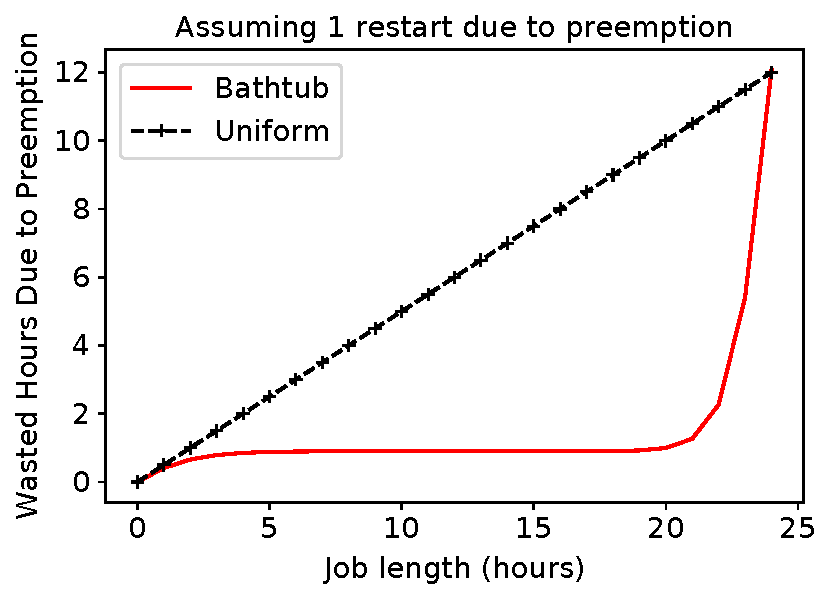
\includegraphics[width=0.23\textwidth]{../graphs/uniform-v-bathtub.pdf} }
 % \\
 % \vspace*{-0.4cm}
    \subfloat[Expected increase in running time. \label{fig:vs-uniform-2}]
    {  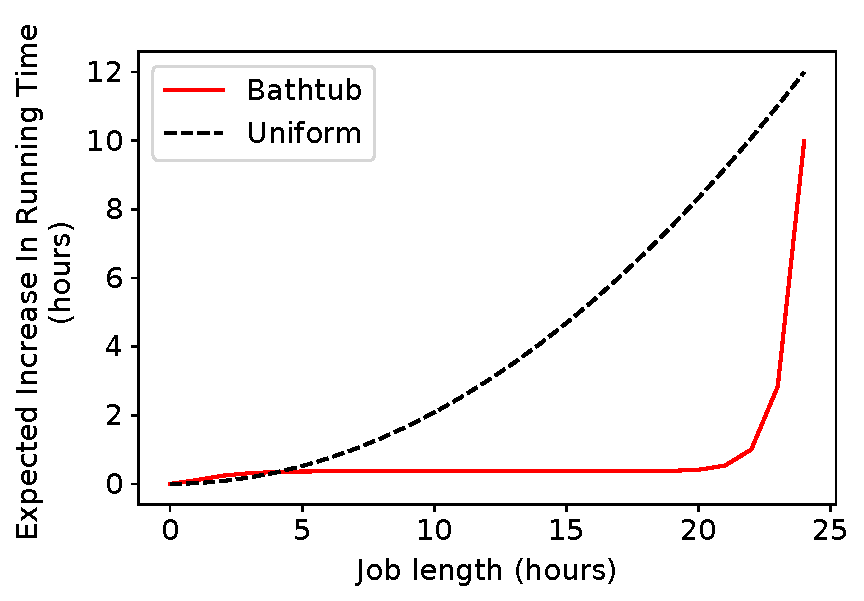
\includegraphics[width=0.23\textwidth]{../graphs/uniform-v-bathtub-2.pdf} }
    \vspace*{-0.4cm}
    \caption{Wasted computation and expected increase in running time for uniform vs. baththub failures. For jobs $>5$ hours, bathtub distribution results in significantly lower wasted computation.}
\vspace*{\myfigspace}    
  \label{fig:vs-uniform-both}
  
\end{figure}

%\caption{The expected wasted computation, given a single failure, is lower when preemptions are distributed in a bathtub shape, compared to uniformly distributed over the 24 hour interval}

We begin by examining how constrained preemptions impacts the total job running times. 
When a preemption occurs during the job's execution, it results in wasted work, assuming there is no checkpointing. 
This increases the job's total expected running time, since it must restart after a preemption.
In case of constrained preemptions, the expected waste depends both on the probability of job preemption, as well as \emph{when} the job was preempted. 


For a job of length $J$, the wasted work, assuming that the job faces a \emph{single} preemption, is $E[W_1(J)]$, and is given by Equation~\ref{eq:wasted}.
We first analyze this wasted work for jobs of different lengths in Figure~\ref{fig:vs-uniform}. 
We analyze two failure probability distributions for constrained preemptions: a uniform distribution such that $F(t) = 24-t$, and the bathtub shaped distribution with parameters corresponding to the \texttt{n1-highcpu-16} VM type shown in Figure~\ref{fig:gcp1}. 


For the uniform distribution, the wasted work is linear in the job length, and is given by $J/2$.
For the bathtub distribution, the wasted work is given by Equation~\ref{eq:wasted}.
% \vikram{
%We find that compared to the uniform case, the bathtub distribution yields on average XXX hours smaller waste for jobs longer than 5 hours, a significant reduction in the wasted work.  %\emph{significantly} lower, especially for longer jobs (longer than 5 hours). 
%With the bathtub distribution, jobs see a high rate of failure initially, but that also reduces the wasted work. 
%Once jobs survive the initial high failure rate, the rate of failure is low, and thus the wasted work is more or less constant for all but the shortest and longest jobs. 
We now examine the expected increase in running time, that also accounts for the probability of failure, and is given by $P(\text{failure})*E[W_1]$. 
Figure~\ref{fig:vs-uniform-2} shows this expected increase in running times for jobs of different lengths.
We see that for uniformly distributed preemptions, the increase in running time is quadratic in the job length (and is given by $J^2/48$). 
Interestingly, the high rate of early failures for the bathtub distribution results in a slightly worse (i.e., higher) running time for short jobs, because of the high initial rate of bathtub preemptions. 
%hl
However for jobs longer than 5 hours, a cross-over point is reached, and the bathtub distribution provides lower overhead of preemptions.
%hl
For instance, for a 10 hour job, the increase in running time is about 30 minutes, or 5\%. 
In comparison, if failures were uniformly distributed, the increase would be 2 hours. 


%hl
Thus, the bathtub preemptions are beneficial for applications and users, as the low failure rate during the middle periods results in significantly lower wasted work (between $1\times--40\times$), compared to the uniformly distributed failures.
%hl 
Since the failure rate distribution is ultimately controlled by the cloud provider, our analysis can be used to determine the appropriate preemption distribution based on the job length distributions.
For instance, if short jobs are very common, then uniformly distributed preemptions are preferable, otherwise, bathtub distributions can offer significant benefits. 

%\noindent \textbf{Result:} \emph{For constrained preemptions, bathtub distributions reduce the expected increase in running times for medium to long running jobs ($5-15$ hours) by up to $40\times$, but are slightly inferior for short jobs ($<5$ hours).}
%hl
%\noindent \textbf{Result:} \emph{Bathtub distributions are beneficial for medium and long duration ($5-15$ hours) jobs, and can reduce the expected increase in running time by up to $40\times$.} 
%hl  
  
\end{comment}


%%%%%%%%%%%%%%%%%%%%%%%%%%%%%%%%%%%%%%%%%%%%%%%%%%%%%%%%%%%%%%%%%%%%%%
\vspace*{\subsecspace}
\subsection{Model-based Policies}
\label{subsec:eval-policy}

We now evaluate the effectiveness of model-driven policies that we proposed earlier in Section~\ref{sec:policies}.
%
Wherever applicable, we compare against policies designed for EC2 spot instances~\cite{harlap2018tributary, spoton} that have memoryless preemptions. 
%
However we also note that certain resource management challenges such as the preemption-rate aware job scheduling are \emph{inherent} to constrained preemptions, and no existing equivalent policies can be found for memoryless techniques. 


%Specifically, we seek to compare the effectiveness of our job scheduling and checkpointing policies with existing transient computing approaches.


\vspace*{\subsecspace}
\subsubsection{Job Scheduling}

Previously, we have quantified the increase in running time due to preemptions, but we had assumed that jobs start on a newly launched server.
In many scenarios however, a server may be used for running a long-running sequence of jobs, such as in a batch-computing service. 
%
Our job scheduling policy is model-driven and decides whether to request a new VM for a job or run it on an existing VM.
A new VM may be preferable if the job starts running near the VM's 24 hour preemption deadline.
%However, since new VMs have a high initial rate of failure, we must be judicious 

Figure~\ref{fig:sched-bathtub} shows the effect of our job scheduling policy for a six hour job, for different job starting times (relative to the VM's starting time). 
We compare against a baseline of memoryless job scheduling that is not informed by constrained preemption dynamics.
Such memoryless policies are the default in existing transient computing systems such as SpotOn~\cite{spoton}. 
In the absence of insights about bathtub preemptions, the memoryless policy continues to run jobs on the existing VM. 
As the figure shows, the empirical job failure probability is bathtub shaped. 
However since the job is 6 hours long, with the memoryless policy, it will always fail when launched after $24-6=18$ hours.
%hl 
In contrast, our model-based policy determines that after 18 hours, we will be better off running the job on a newer VM, and results in a constant lower job failure probability (=0.4). The failure probability is constant because the jobs will always be launched on a new VM after 18 hours, resulting in a failure probability at time=0. 
%hl
Thus, our model-based job scheduling policy can reduce job failure probability by taking into account the time-varying failure rates of VMs, which is not considered by existing systems that use memoryless scheduling policies. 

%%%%%%%%%%%%%%%%%%%%%%%%%%%%%%%%%%%%%%%%

%\textbf{Tipping points:}



% \begin{figure*}
%   \centering
%   \begin{minipage}[c]{0.3\linewidth}
%     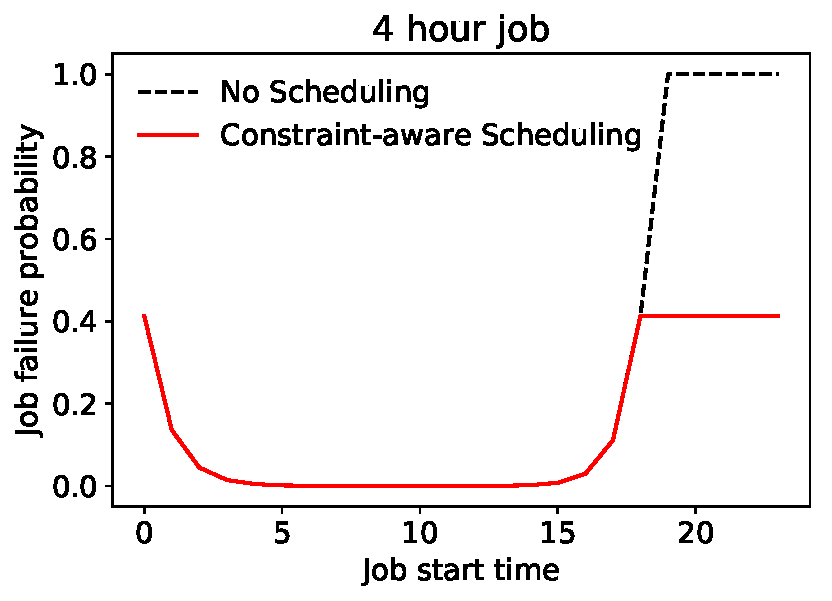
\includegraphics[width=\linewidth]{../graphs/Sched-bathtub.pdf}
%     \vspace*{-0.6cm}
%     \caption{Effect of job start time on the failure probability.} \label{fig:sched-bathtub}
%   \end{minipage}
% %  \caption{Our model-driven job-scheduling policy reduces job-failures.}
% %  \label{fig:sched-top}
%   \hfill 
%   \begin{minipage}[c]{0.3\linewidth}
%     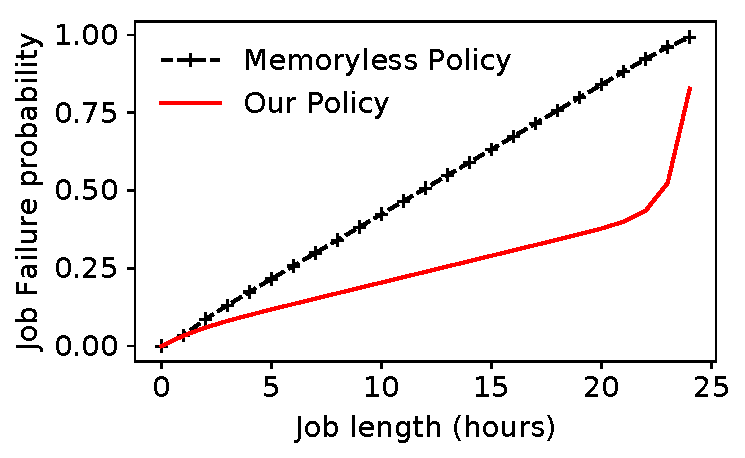
\includegraphics[width=\textwidth]{../graphs/Sched-fail-prob.pdf}
%     \vspace*{-0.6cm}
%     \caption{Job failure probability for jobs of different lengths.} \label{fig:sched-all}
%   \end{minipage}
%   \hfill
% \begin{minipage}[c]{0.3\textwidth}
%   \centering
%   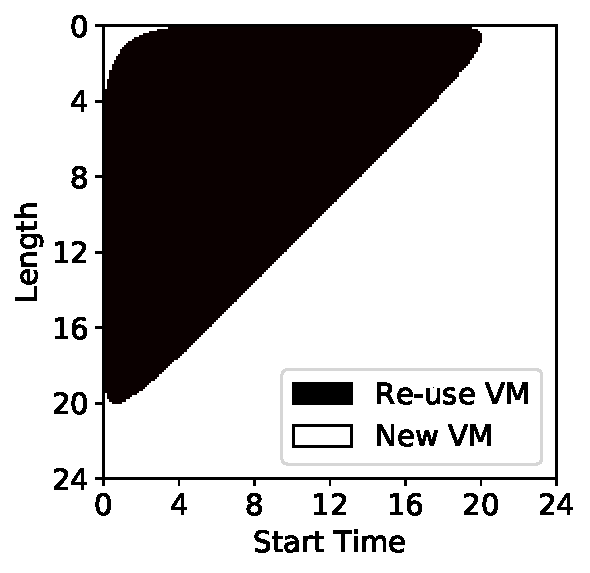
\includegraphics[width=0.7\textwidth]{../graphs/tipping-black-reuseVM.pdf}
%   \caption{Job lengths and starting points where VM should be reused (black), and a new VM should be launched (white)}
%   \label{fig:tipping-points}
% \end{minipage}

  
%   \begin{minipage}[c]{0.3\linewidth}
%     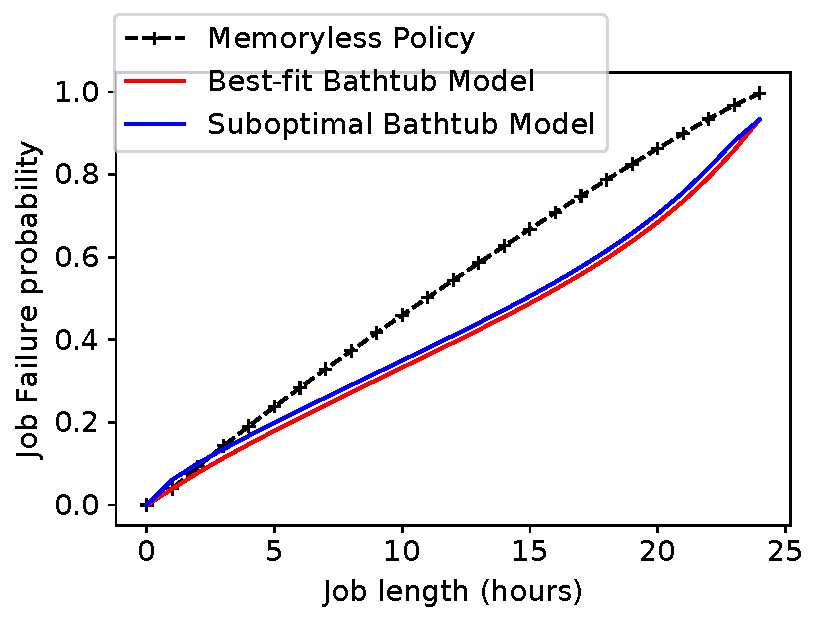
\includegraphics[width=\linewidth]{../graphs/wrong-model.pdf}
%     \vspace*{-0.8cm}
%   \caption{Impact of suboptimal bathtub model parameters on the scheduling policy is negligible.}
%   \label{fig:wrong-model}
% \end{minipage}
%\vspace*{-0.4cm}
%\end{figure*}


\begin{figure}[t]
  \vspace*{\myfigspace}
  \subfloat[Effect of job start time on the failure probability. \label{fig:sched-bathtub}]
  {  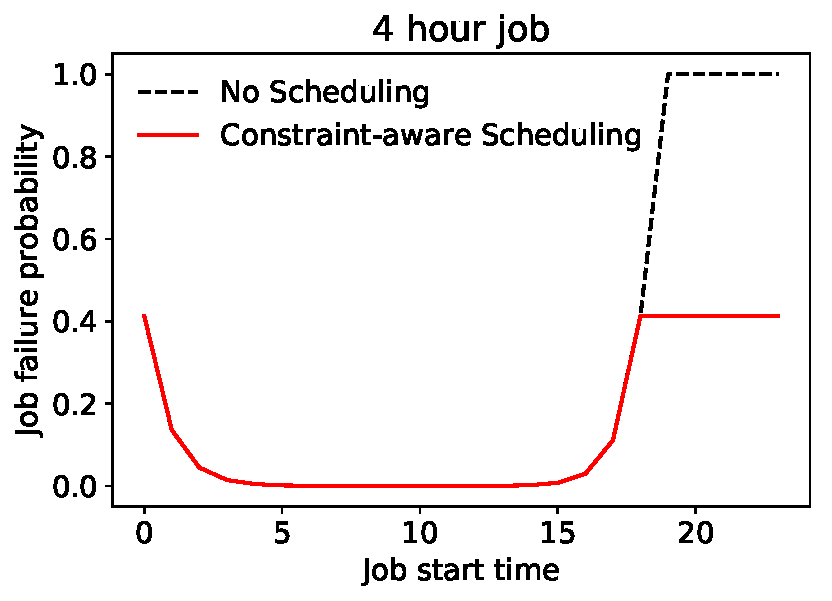
\includegraphics[width=0.23\textwidth]{../graphs/Sched-bathtub.pdf}}
  \hfill
  \vspace*{-0.4cm}
  \subfloat[Job failure probability for jobs of different lengths. \label{fig:sched-all}]
  {  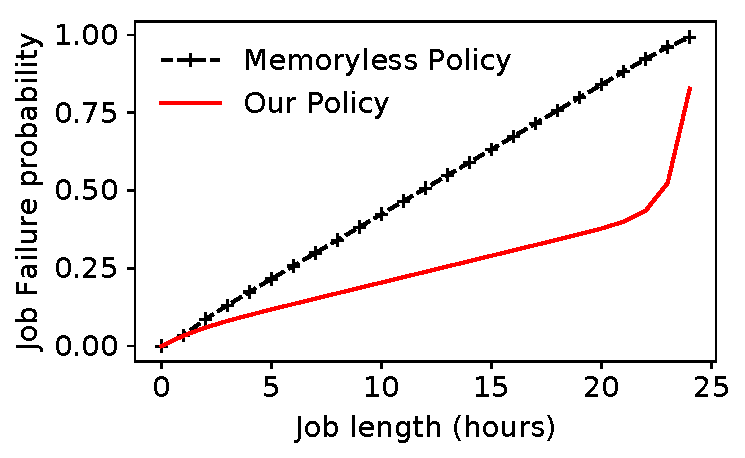
\includegraphics[width=0.23\textwidth]{../graphs/Sched-fail-prob.pdf}}
  %  \vspace*{\myfigspace}
  \caption{Job failure probability is lower with our deadline aware policy across all job sizes.}
  \vspace*{\myfigspace}
  \label{fig:sched-both}
\end{figure}


The job failure probability is determined by the job length and the job starting time.
%hl
We examine the failure probability for jobs of different lengths (uniformly distributed) in Figure~\ref{fig:sched-all}, in which we average the failure probability across different start times.
%hl 
We again see that our policy results in significantly lower failure probability compared to memoryless scheduling.
For all but the shortest and longest jobs, the failure probability with our policy is \emph{half} of that of existing memoryless policies. 
This reduction is primarily due to how the two policies perform for jobs launched near the end of the VM preemption deadline, which we examined previously in Figure~\ref{fig:sched-bathtub}. 

%hl repeats previous sentence anyway. 
%\noindent \textbf{Result:} \emph{Our model-based job scheduling and VM-reuse policy can decrease job failure probability by up to $2\times$ for medium and long jobs.}
%hl

% \begin{figure}
%   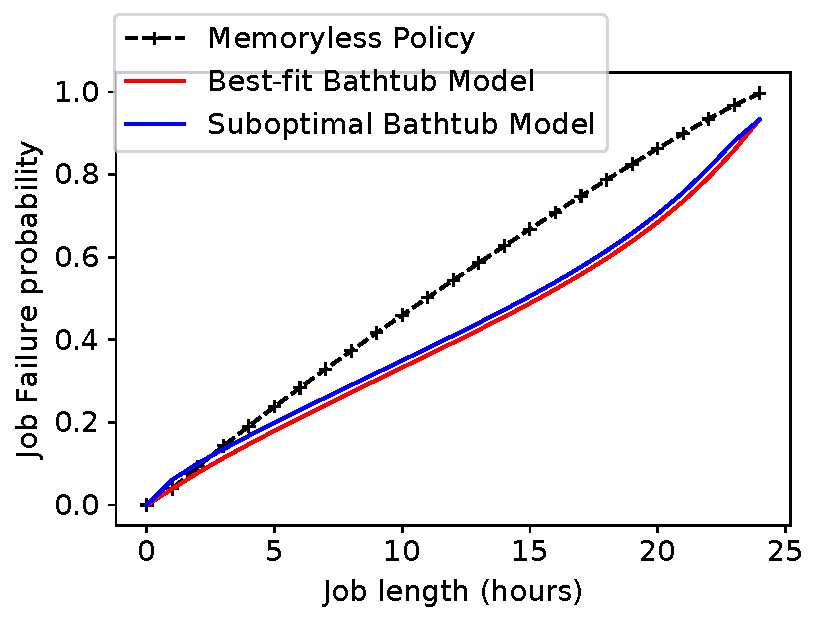
\includegraphics[width=0.3\textwidth]{../graphs/wrong-model.pdf}
%   \caption{Impact of choosing  ``wrong'' bathtub model parameters on the scheduling policy is negligible.}
%   \label{fig:wrong-model}
% \end{figure}

\begin{comment}

\noindent \textbf{Sensitivity to model fitting.}
The effectiveness of any model-based policy depends on the goodness of fit of the preemption model---i.e., how accurately it captures empirical data. 
%
We now evaluate the impact on our scheduling policy if incorrect/suboptimal model parameters are with high goodness-of-fit ($r^2$) error are used. 
%
That is, we seek to understand how sensitive our policies are when the underlying preemption behavior does not match the model, which can occur due to changes in supply/demand, minor cloud policy changes, etc. 
%
Figure~\ref{fig:wrong-model} compares the job failure probability with the optimal bathtub model that best fits the empirical data, and a suboptimal  bathtub model intentionally chosen to have a bad fit. 
%
Specifically, the suboptimal case models the \texttt{n1-highcpu-16} VMs for \texttt{n1-highcpu-32} VMs, which from Figure~\ref{fig:cdf-comparison} we can see are significantly different.
%
However even with the suboptimal model, the increase in job failure probability is less than 2\% compared to the best-fit model. 
%
This negligible difference is due to the fact that even a suboptimal model captures the bathtub shape, and this is enough for the policy to make the ``right'' scheduling decision. 

\noindent \textbf{Result:} \emph{Our policies are not particularly sensitive to the exact model parameters, so long as a bathtub distribution is used. Even a suboptimal bathtub model can reduce failure probability by 15\% compared to the memoryless policy.} 
%
%This is desirable in cloud environments where the underlying preemption distribution can change, and thus our empirical model driven approach is a feasible technique for harnessing temporally constrained VMs. 

\end{comment}

    
\begin{comment}
%%%%%%%%%%%%%%%%%%%%%%%%%%%%%%%%%%%%%%%%%%%%%%%%%%
\vspace*{\subsecspace}
\subsubsection{Checkpointing}
\label{subsec:eval-ckpt}

We now evaluate our model-based checkpointing policy, that uses a dynamic programming approach.
With our policy, the checkpointing rate is determined by the VM's current failure rate.
In contrast, all prior work in transient computing and most prior work in fault-tolerance assumes that failures are exponentially distributed (i.e., memoryless), and use the Young-Daly checkpointing interval.
In the Young-Daly approach, checkpoints are taken after a constant period given by $\tau \propto \sqrt{MTTF}$.
%
However in the case of constrained preemptions with bathtub distributions, the failure rate is time-dependent and not memoryless. 


The expected increase in running time for a 4 hour job is shown in Figure~\ref{fig:ckpt-4}, in which we account for both the increase due to the checkpointing overhead, as well as the expected recomputation due to preemptions. 
Throughout, we assume that each checkpoint takes 1 minute. 
The increase in running time depends on the failure rate and thus the job's starting time. 
With our model-based checkpointing policy, the increase in running time is bathtub shaped and is below 5\%, and around 1\% when the job is launched when the VM is between 5 and 15 hours old. 

We also compare with the Young-Daly~\cite{daly2006higher} periodic checkpointing policy, as implemented in~\cite{flint, proteus-eur17, marathe2014exploiting}, and which represents the broad class of fault-tolerance techniques proposed for transient computing. 
%
For Young-Daly, we use the initial failure rate of the VM to determine the MTTF, which corresponds to an MTTF of 1 hour. 
This results in a high, constant rate of checkpointing, and increases the running time of the job by more than 25\%.
The increase in running time is primarily due to the overhead of checkpointing. 
Note that checkpointing with a lower frequency decreases the checkpointing overhead, but increases the recomputation required.

Next, we examine the expected running time of jobs of different length, when all jobs start at time=0, i.e, are launched on a freshly launched VM.
%hl
Figure~\ref{fig:ckpt-start-0-relative} shows the expected increase in the running time of the jobs of length $(0-9] $ hours, with our model-based checkpointing policy and the Young-Daly policy with MTTF=1 hour.
%hl 
With our policy, the running times increase by 10\% for short jobs ($<2$  hours), and increase by less than 5\% for longer jobs, staying at 3\% on average. 
In contrast, the Young-Daly policy yields a constant increase in running times of 25\%. 
Thus, our model-based policy is able to reduce the checkpointing overhead and thus reduce the performance overhead of running on preemptible VMs to below 5\%. 

\noindent \textbf{Result:} \emph{Our checkpointing policy can keep the performance overhead of preemptions under 5\%, which is $5\times$ better than conventional periodic checkpointing.}


\begin{figure}[t]
  \vspace*{\myfigspace}
  \subfloat[Checkpointing overhead for different job starting times. \label{fig:ckpt-4}]
{  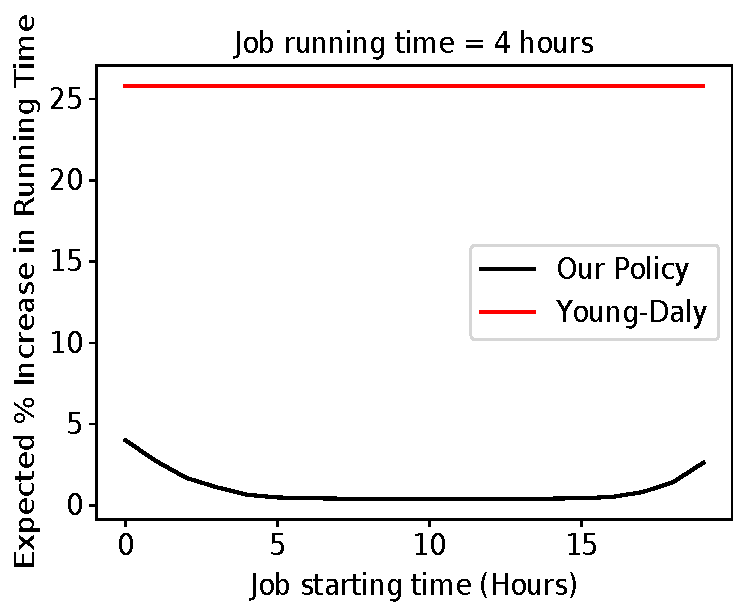
\includegraphics[width=0.23\textwidth]{../graphs/ckpt-4-trim.pdf} }
%\hfill
% \subfloat[Running time with checkpointing when jobs start at time=0. \label{fig:ckpt-start-0}]
% {  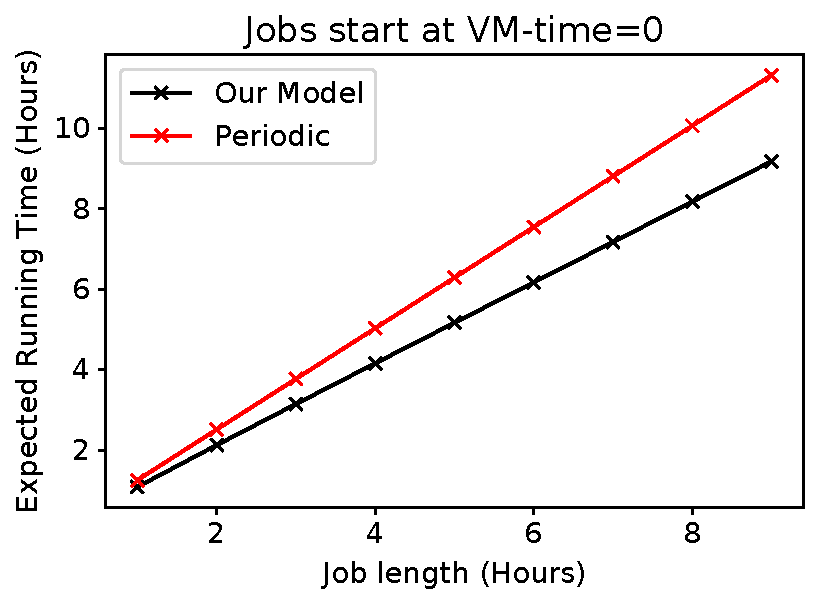
\includegraphics[width=0.3\textwidth]{../graphs/ckpt-start-0.pdf}}
% \hfill
%\\
%\vspace*{-8pt}
\subfloat[Increase in running time with checkpointing when jobs start at time=0. \label{fig:ckpt-start-0-relative}]
{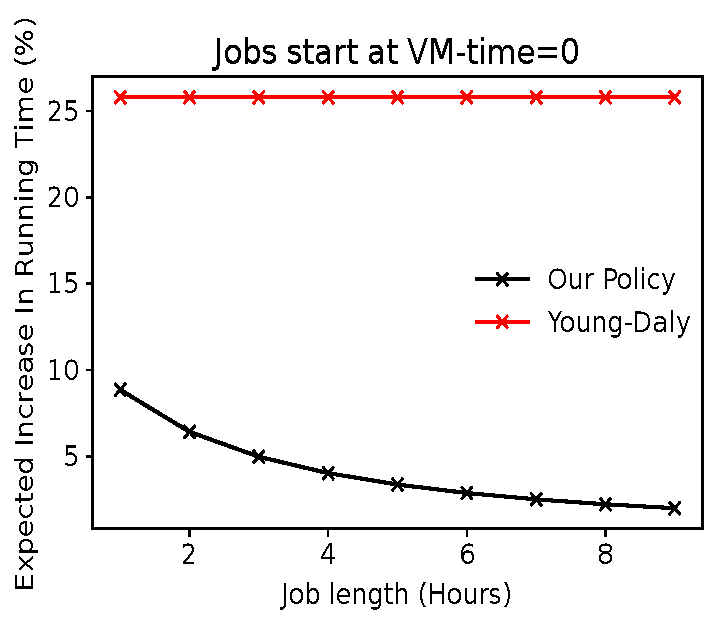
\includegraphics[width=0.23\textwidth]{../graphs/ckpt-start-relative-trim.pdf}}
\vspace*{\myfigspace}
  \caption{Checkpointing effectiveness.}
  \label{fig:ckpt-all}
  \vspace*{-0.3cm}
\end{figure}

\end{comment}

%%%%%%%%%%%%%%%%%%%%%%%%%%%%%%%%%%%%%%%%

\subsubsection{Impact of server exploration}

%As described in Section~\ref{sec:design}, applications can be deployed on multiple types of VMs in the cloud, with each VM type having a different ``size''.
%In our evaluation of parallel scientific computing applications that are CPU intensive, we are primarily interested in the number of CPUs in a VM.

When an application (i.e., bag of jobs) requests a total number of CPUs to run each of its jobs, \sysname first runs its exploration phase to find the ``right'' VM for the application.
\sysname searches for the VM that minimizes the total expected cost $E[C_{(i,n_i)}]$ of running the application. %and this depends on several factors such as the parallel structure of the application, the preemption probability and the associated job recomputation time, and the price of the VM.
Thus, even if the \emph{total} amount of resources (i.e., number of CPUs) per job is held constant, the total running time (i.e., turnaround time) of an application depends on the choice of the VM type ($i$), and the associated number of VMs ($n_i$) required to meet the allocation constraint (Section~\ref{subsec:cost-model}).
%
With preemptible instances, the total running time of a job is composed of two factors: the ``base'' running time of the job without any preemptions ($T_{(i,n_i)}$), and the expected recomputation time which depends on the probability of job failure (Equation~\ref{eq:recomput}). 

\begin{figure}
  \centering
  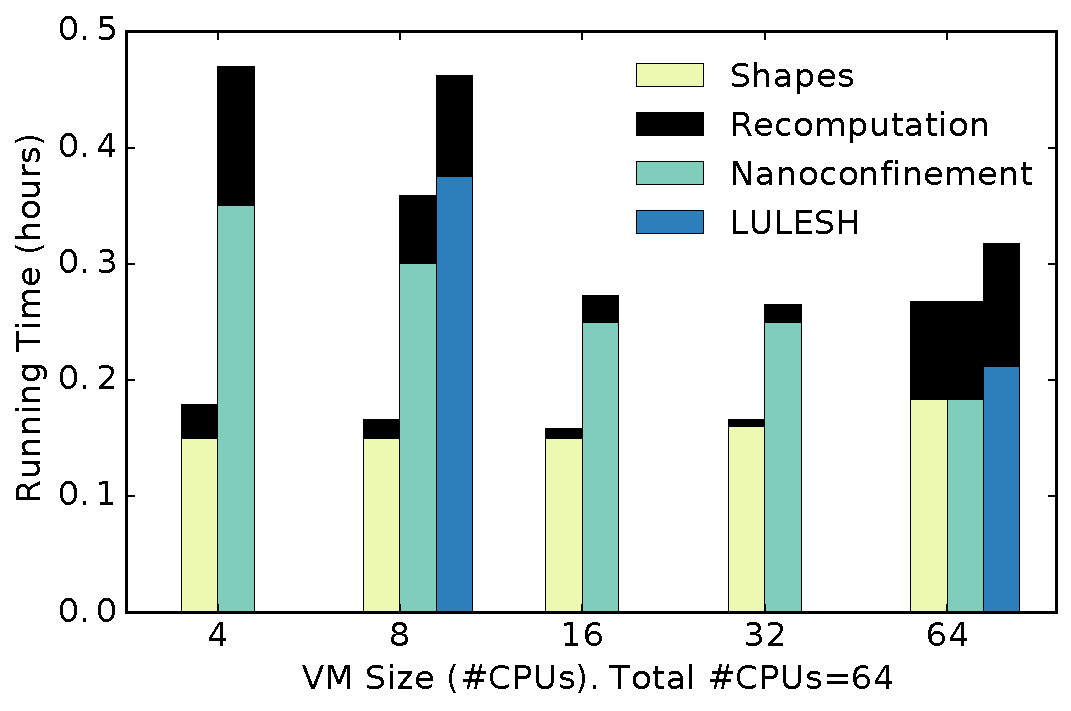
\includegraphics[width=0.4\textwidth]{../graphs/runtime-bars.pdf}
      \vspace*{\myfigspace}
  \caption{Running times of applications on different VMs. Total number of CPUs is 64, yielding different number of VMs in each case. We see different tradeoffs in the base running times and recomputation times.}
  \label{fig:runtimes-bar}
    \vspace*{\myfigspace}
\end{figure}


Figure~\ref{fig:runtimes-bar} shows the running times of the Nanoconfinement, Shapes, and LULESH applications, when they are deployed on different VM sizes. 
In all cases, the total number of CPUs per job is set to 64, and thus the different VM sizes yield different cluster sizes (e.g., 16 VMs with 4 CPUs or 32 VMs with 2 CPUs).
LULESH requires CPUs to be cube of an integer, which limits the valid cluster configurations. 

For Nanoconfinement and LULESH, we observe that the base running times (without preemptions) reduce when moving to larger VMs, because this entails lower communication costs.
For Nanoconfinement, the running time on the ``best'' VM (i.e., with 32 CPUs) is nearly 40\% lower as compared to the worst case. 
On the other hand, the Shapes application can scale to a larger number of VMs without any significant communication overheads, and does not see any significant change in its running time. 

Figure~\ref{fig:runtimes-bar} also shows the expected turnaround time $E[\mathcal{T}_{(i,n_i)}]$, that is obtained by adding the the expected recomputation time, which depends on the expected lifetimes of the VM and the number of VMs, and is computed using the cost model introduced in Section~\ref{subsec:cost-model}. 
While selecting larger VMs may reduce communication overheads and thus improve performance, it is not an adequate policy in the case of preemptible VMs, since the preemptions can significantly increase the turnaround time.
Therefore, even though the base running time of Nanoconfinement is lower on a 64 CPU VM, the recomputation time on the 64 CPU VM is almost $4\times$ higher compared to a 2x32-CPU cluster,  due to the much lower expected lifetime of the larger VMs. 
Thus, on preemptible servers, there is a tradeoff between the base running time which only considers parallelization overheads, and the recomputation time.
By considering \emph{both} these factors, \sysname's server selection policy can select the best VM for an application. 


\noindent \emph{\textbf{Result:} SciSpot's server selection, by considering both the base running time and recomputation time, can improve performance by up to 40\% , and can keep the increase in running time due to recomputation to less than 5\%.}

%%%%%%%%%%%%%%%%%%%%%%%%%%%%%%%%%%%%%%%%%%%%%%%%%%
\subsubsection{Cost}


\begin{figure}
  \centering
  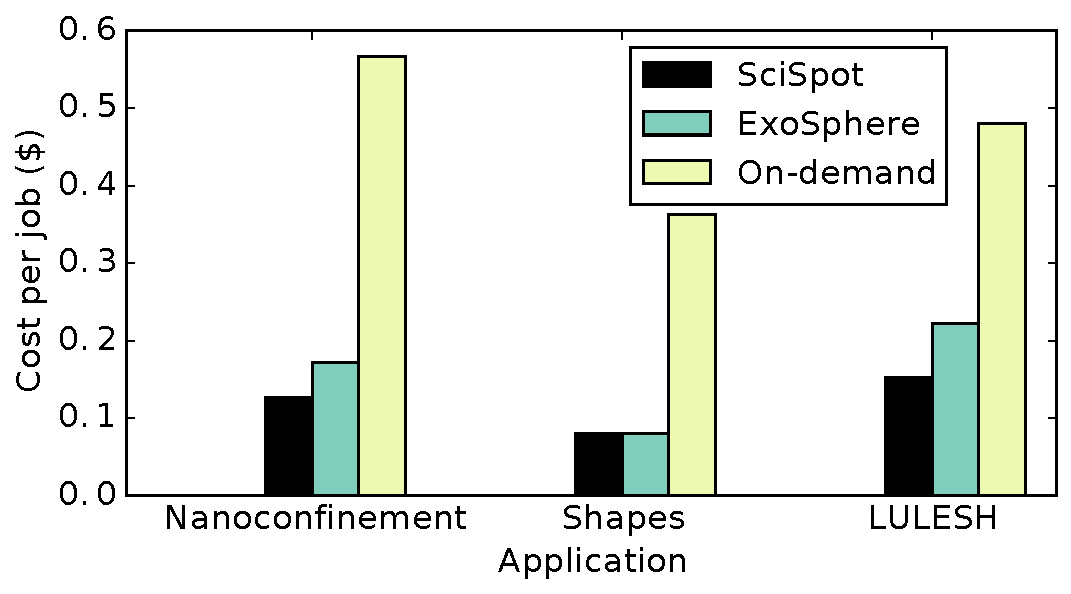
\includegraphics[width=0.4\textwidth]{../graphs/cost-vs-exosphere.pdf}
  \vspace*{\myfigspace}
  \caption{SciSpot's use of preemptible VMs can reduce costs by up to $5\times$ compared to conventional cloud deployments, and 20\% compared to the state of the art EC2 spot instance selection (ExoSphere~\cite{exosphere}).}
  \label{fig:cost-only-bar}
    \vspace*{\myfigspace}
\end{figure}

The primary motivation for using preemptible VMs is their significantly lower cost compared to conventional ``on-demand'' cloud VMs that are non-preemptible. 
Figure~\ref{fig:cost-only-bar} compares the cost of running different applications with different cloud VM deployments. 
\sysname, which uses both cost-minimizing server selection, and preemptible VMs, results in significantly lower costs across the board, even when accounting for preemptions and recomputations. 
%
We also compare against ExoSphere~\cite{exosphere}, a state of the art  system for transient server selection.
ExoSphere implements a portfolio-theory approach using EC2 spot prices to balance average cost saving and risk of revocations using diversification and selecting VMs with low price correlation.
However, this approach is ineffective for the flat prices of Google Preemptible VMs. 
Unlike \sysname, ExoSphere does \emph{not} consider application performance when selecting servers, and thus is unable to select the best server for parallel applications. 
Since the Google \texttt{highcpu} VMs have the same price per CPU, ExoSphere picks an arbitrary ``median'' VM to break ties, which may not necessarily yield the lowest running times.
This results in 20\% cost increase over \sysname. 

\noindent \emph{\textbf{Result:} SciSpot reduces computing costs by up to 5$\times$ compared to conventional on-demand cloud deployments.}


\eat{
\begin{figure}
  \centering
  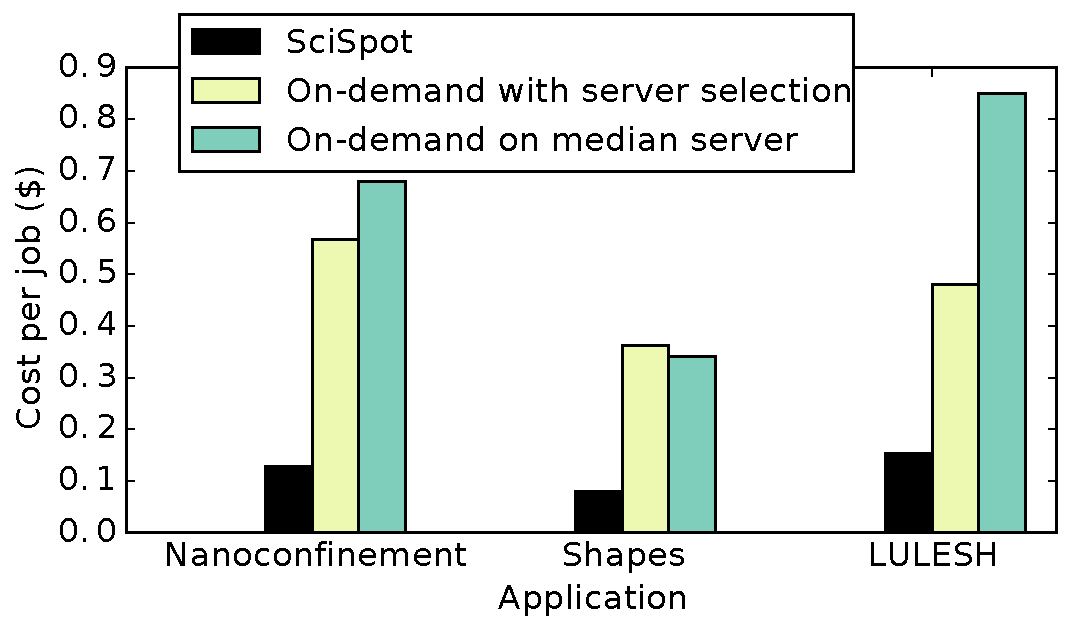
\includegraphics[width=0.4\textwidth]{../graphs/cost-only-bar.pdf}
  \vspace*{\myfigspace}
  \caption{SciSpot's use of preemptible VMs can reduce costs by up to $5\times$ compared to conventional cloud deployments.}
  \label{fig:cost-only-bar}
    \vspace*{\myfigspace}
\end{figure}

The primary motivation for using preemptible VMs is their significantly lower cost compared to conventional ``on-demand'' cloud VMs that are non-preemptible. 
Figure~\ref{fig:cost-only-bar} compares the cost of running different applications with different cloud VM deployments.
\sysname, which uses both cost-minimizing server selection, and preemptible VMs, results in significantly lower costs across the board, even when accounting for preemptions and recomputations. 
Even with \sysname's server selection, using on-demand VMs result in a $5\times$ cost increase compared to \sysname.
In the absence of server selection, we assume that the user will pick a ``median'' VM in terms of number of CPUs (in this case, 8 CPU VMs), which we also show in Figure~\ref{fig:cost-only-bar}.
Note that since \sysname's server selection considers the turnaround time (which includes recomputation time), it may not always pick the optimal on-demand server. 

\noindent \emph{\textbf{Result:} SciSpot reduces computing costs by up to 5$\times$ compared to conventional on-demand cloud deployments.}
}
%%%%%%%%%%%%%%%%%%%%%%%%%%%%%%%%%%%%%%%%%%%%%%%%%%
\subsubsection{Comparison with HPC Overhead}

Scientific computing applications are typically run on large-scale HPC clusters, where different performance and cost dynamics apply.
While there are hardware differences between cloud VMs and HPC clusters that can contribute to performance differences, we are interested in the performance ``overheads''.
In the case of \sysname, the job failures and recomputations increase the job turnaround time, and are thus the main source of overhead.

On HPC clusters, jobs enjoy significantly lower recomputation probability, since the hardware on these clusters has MTTFs in the range of years to centuries~\cite{dongarra_fault_nodate}.
However, we emphasize that there exist \emph{other} sources of performance overheads in HPC clusters.
In particular, since HPC clusters have high resource utilization, they also have significant \emph{waiting} times. 
On the other hand, cloud resource utilization is low~\cite{borg} and there is usually no need to wait for resources, which is why transient servers exist in the first place. 


Thus, we compare the performance overhead due to preemptions for \sysname, and job waiting times in conventional HPC deployments.
To obtain the job waiting times in HPC clusters, we use the LANL Mustang traces published as part of the Atlas trace repository~\cite{cmu-atlas}.
We analyze the waiting time of over two million jobs submitted over a 5 year period, and compute the increase in running time of the job due to the job waiting or queuing time. 

\begin{figure}[t]
  \centering 
  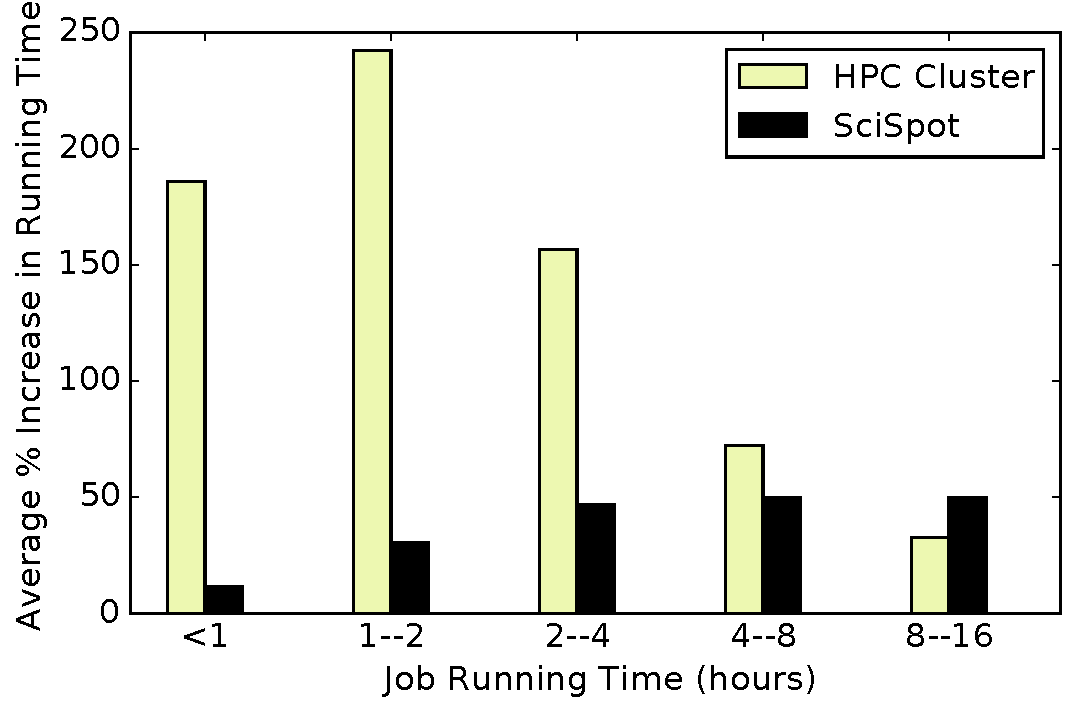
\includegraphics[width=0.4\textwidth]{../graphs/hpc-vs-scispot.pdf}
      \vspace*{\myfigspace}
  \caption{Increase in running time due to waiting on HPC clusters is significantly higher than the recomputation time for \sysname, except for very long and rare jobs (see inset). }
  \label{fig:hpc-vs-scispot}
  \vspace*{\myfigspace}
\end{figure}


%We define the overhead as the increase in running time which is equal to the turnaround time (i.e., the time between the job submission and successful completion) divided by the base job running time (with no waiting or premptions). 
%In HPC clusters, the overhead is the waiting time for resources, and in \sysname the overhead is the recomputation time due to preemptions.
Figure~\ref{fig:hpc-vs-scispot} compares the overhead (as percentage increase in running time) of \sysname and HPC clusters  for jobs of different lengths. We see that the average performance overhead due to waiting can be significant in the case of HPC clusters, and the job submission latency and queuing time dominate for smaller jobs, increasing their total turnaround time by more $2.5\times$.
This waiting is amortized in the case of longer running jobs, and the overhead for longer jobs is around 30\%.

On the other hand, \sysname's performance overhead is significantly smaller for jobs of up to 8 hours in length.
For longer jobs, the limited lifetime of Google Preemptible VMs (24 hours) begins to significantly increase the preemption probability and expected recomputation time.
We emphasize that these are \emph{individual} job lengths, and not the running time of entire bag of jobs.
We note that these large single jobs are rare, accounting for less than 5\% of all HPC jobs (see inset in Figure~\ref{fig:hpc-vs-scispot}).
For smaller jobs (within a much larger bag), both the preemption probability and recomputation overhead is much smaller. 

\noindent \emph{\textbf{Result:} \sysname's overhead of recomputation due to preemptions is small, and is up to $10\times$ lower compared to the overhead of waiting in conventional HPC clusters. }







%%%%%%%%%%%%%%%%%%%%%%%%%%%%%%%%%%%%%%%%%%%%%%%%%%

\begin{comment}
%\subsection{SciSpot Evaluation}
\vspace*{\subsecspace}
\subsection{Effectiveness on Scientific Computing Workloads}

We now show the effectiveness of our batch computing service on Google Preemptible VMs.
We run scientific simulation workloads described earlier in this section, and are interested in understanding the real-world effectiveness of our model-based service.
%We use our model-driven job scheduling policy, but do not use checkpointing, since it requires additional application modifications. 

%%%%%%%%%%%%%%%%%%%%%%%%%%%%%%%%%%%%%%%%%%%%%%%%%%


%As described in Section~\ref{sec:design}, applications can be deployed on multiple types of VMs in the cloud, with each VM type having a different ``size''.
%In our evaluation of parallel scientific computing applications that are CPU intensive, we are primarily interested in the number of CPUs in a VM.


%%%%%%%%%%%%%%%%%%%%%%%%%%%%%%%%%%%%%%%%%%%%%%%%%%


\begin{figure}[t]
  \vspace*{\myfigspace}
  \centering
  \subfloat[Cost \label{fig:cost-only-bar}]
{  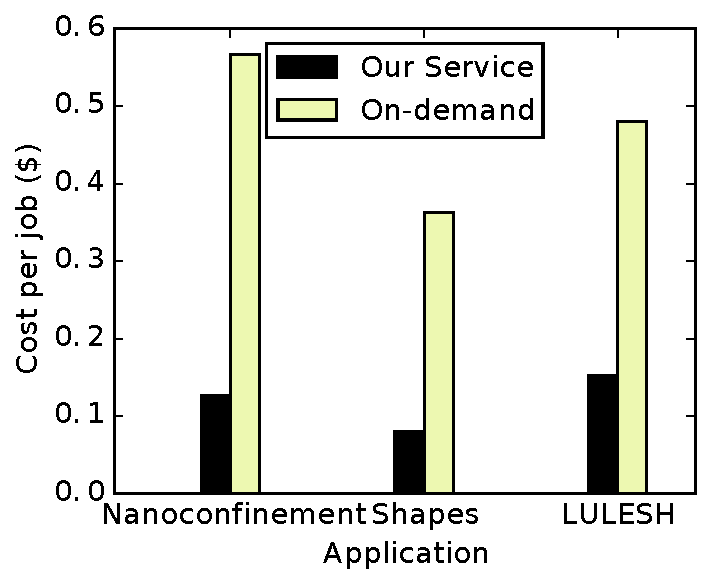
\includegraphics[width=0.25\textwidth]{../graphs/cost-vs-ondem.pdf} }
\hfill
\subfloat[Preemptions \label{fig:fails-time}]
{ 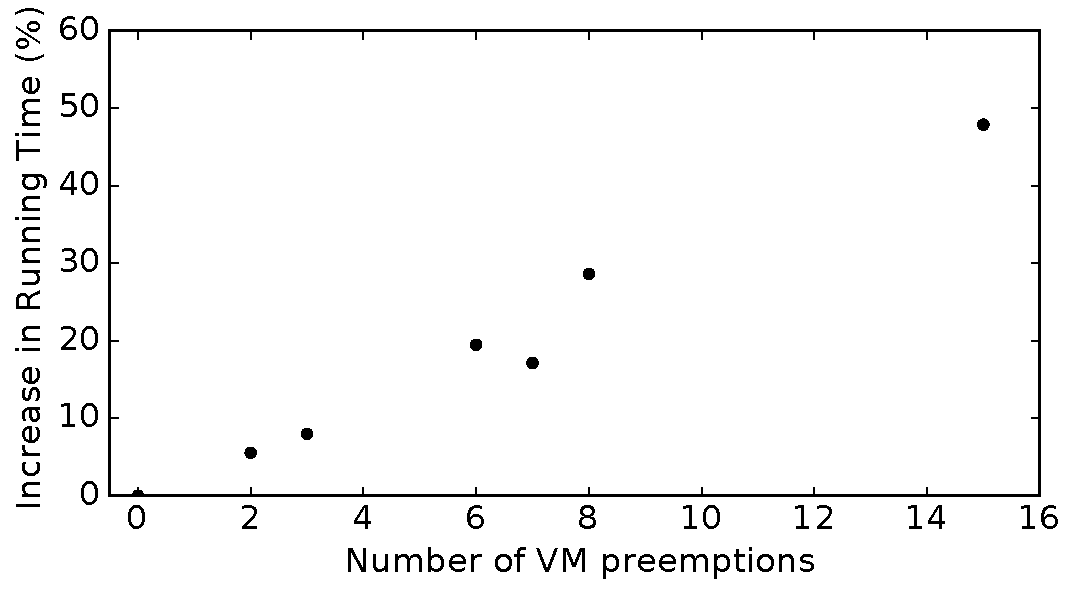
\includegraphics[width=0.2\textwidth]{../graphs/confin-fails-vs-time-relative.pdf} }
\label{fig:service-all}
\vspace*{-0.4cm}
\caption{Cost and preemptions with our service.}
\vspace*{\myfigspace}
\end{figure}  

%  \caption{SciSpot's use of preemptible VMs can reduce costs by up to $5\times$ compared to conventional cloud deployments, and 20\% compared to the state of the art EC2 spot instance selection (ExoSphere~\cite{exosphere}).}
%  \label{fig:cost-only-bar}
%    \vspace*{\myfigspace}


\noindent \textbf{Cost:}
The primary motivation for using preemptible VMs is their significantly lower cost compared to conventional ``on-demand'' cloud VMs that are non-preemptible.
To evaluate the cost of using our batch computing service, we run a bag of 100 jobs, all running on a cluster of 32 VMs of type \texttt{n1-highcpu-32}. 
Within a bag, different jobs are exploring different physical parameters, and job running times show little variance. 
Figure~\ref{fig:cost-only-bar} shows the cost of using Preemptible VMs compared to conventional on-demand VMs.
We see that our service can reduce costs by $5\times$ for all the applications. % \vikram{you can make this precise by just giving numbers for each application and then saying, on average cost reduction is by 5 times}.

We note that for this experiment, our  service was using model-driven job scheduling, but was not using checkpointing, since the applications lacked checkpointing mechanisms.
Using checkpointing would reduce the costs even further, since it would reduce the increase in running time (and server costs) due to recomputation.


\noindent \textbf{Preemptions:} 
Finally, we examine the effect of preemptions on the increase in running time under real-world settings.
We ran a cluster of 32 \texttt{n1-highcpu-32} VMs running the Nanoconfinement application, and repeated the experiment multiple times to observe the effect of preemptions.
Figure~\ref{fig:fails-time} shows the increase in running time of the entire bag of jobs, when different number of VM preemptions are observed during the entire course of execution.
We see that the net impact of preemptions results in a roughly linear increase in running time. 
Each preemption results in a roughly 3\% increase in running time, which validates our analytical evaluation shown earlier in Figure~\ref{fig:vs-uniform-2}.
% hl
The increase in running time is small because we are computing the \emph{expected} increase in running time, which includes the relatively low probability of preemption. 
%hl 
The result also highlights the effectiveness of the job scheduling and VM-reuse policy, since most jobs run on the stable VMs, and  those that run on new VMs ``fail fast'' and result in only a small amount of wasted work and increase in running time. 


% \begin{figure}[t]
%   \centering 
%         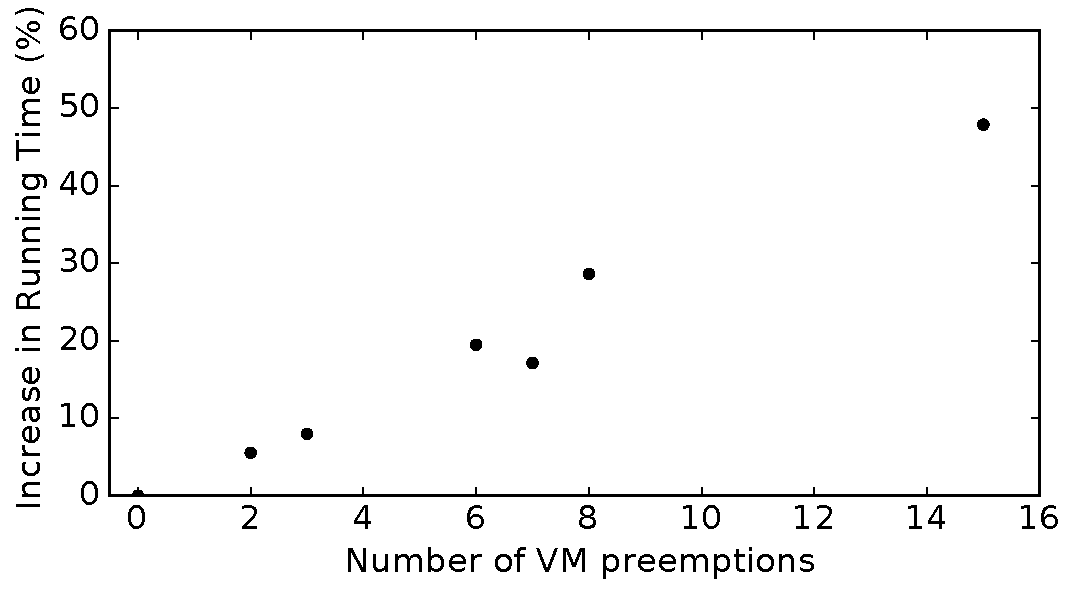
\includegraphics[width=0.22\textwidth]{../graphs/confin-fails-vs-time-relative.pdf}
%       \caption{The increase in running time due to preemptions is under 50\%, even at high preemption rates.}
%         %when the number of preemptions is high.}
%   \label{fig:fails-time}
% \end{figure}


\noindent \emph{\textbf{Result:} Our batch computing service can reduce costs by up to 5$\times$ compared to conventional on-demand cloud VMs. With the VM-reuse policy, the performance impact of preemptions is as low as 3\%.}
  %which is $20\times$ lower than a memoryless policy.}

\end{comment}

%%%%%%%%%%%%%%%%%%%%%%%%%%%%%%%%%%%%%%%%%%%%%%%%%%
%HPC should be the last thing ?


% \begin{figure}
%   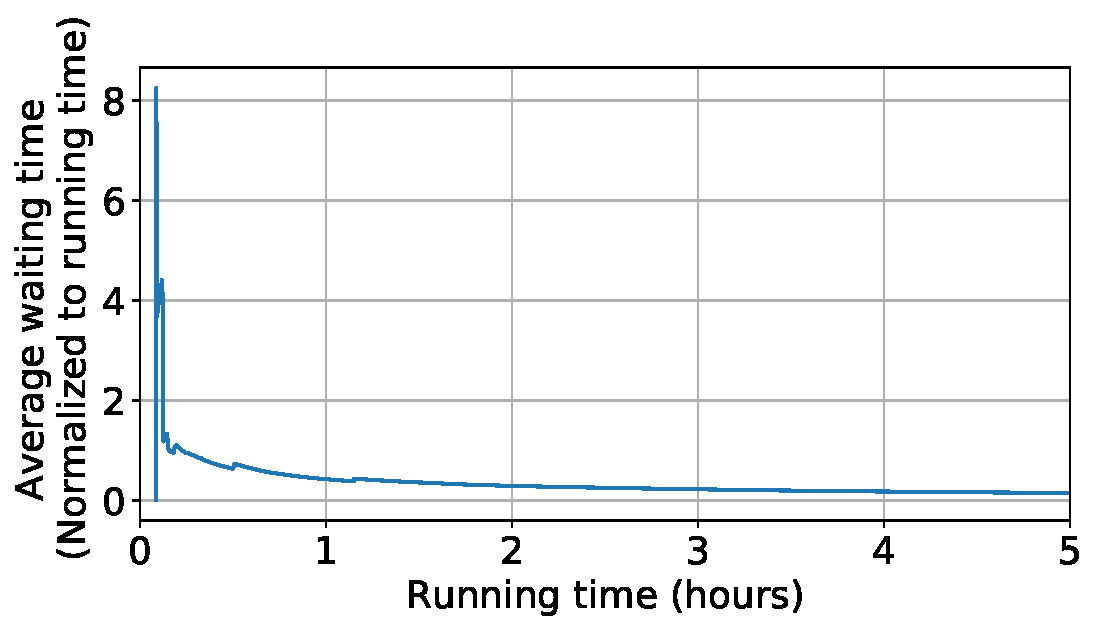
\includegraphics[width=0.4\textwidth]{../data/waiting_cumul.pdf}
%   \caption{The average waiting time (normalized to running time) of jobs of different length.}
%   \label{fig:hpc-wait-cdf}
% \end{figure}



%%% Local Variables:
%%% mode: latex
%%% TeX-master: "paper"
%%% End:
